\documentclass{article}
\usepackage[utf8]{inputenc}
\usepackage{graphicx}
\usepackage{rotating}
\usepackage[a4paper, total={6in, 8in}]{geometry}
\title{Updated assessment of ${\Delta^{14}CO_{2}}$ measurement intercomparability using atmospheric records and standard materials}
\begin{document}
\maketitle


\newpage
\begin{abstract}
Placeholder
\end{abstract}


\newpage
\section{Introduction}
TODO: 
Add a table like that of Miller 2013 Table 1. 
is the NWT3 and NWT4 that I present that same as that of Miller 2013 results? 

\newpage
\section{Methods}
The following institutions' radiocarbon measurements (${\Delta^{14}C}$ and/or FM) 
were compared with the GNS Rafter Radiocarbon Laboratory in turn, each elaborated upon in the following sections. Each intercomparison is tailored specifically to the type of data available between each institution. 
\subsection{Rafter Radiocarbon Lab}
The rafter lab operates the longest running record of atmospheric 14CO2...
\subsection{Heidelberg University}
\subsubsection{Available Data}
The Heidelberg University Institute of Environmental Physics in affiliation with the ICOS Central Radiocarbon Laboratory operates a network of time-series stations measuring ${\Delta^{14}CO_{2}}$
One of these stations, Cape Grim, Tasmania (CGO; 40.68S, 144.68E, 94 m a.s.l; ~\cite{levin2010}), is a reasonable candidate through which to compare Heidelberg University to Rafter Radiocarbon Lab ${\Delta^{14}CO_{2}}$. 

Rafter samples were collected via..., Heidelberg samples were collected via...,

Cape Grim and Baring Head observe a similar mixture of air from the Southern Ocean and Australia ~\cite{ziehn2014}, and a short initial time-series indicates no measurable difference between the sites from 2017-2019 (See Figure \ref{fig:bhdvcgo}). 
Previous analyses has found not much difference in seasonality between the two in overlapping period:~\cite{turnbull2017} see page 14779 FINE TUNE THIS SENTENCE). 
Previously anomalous NaOH data from Rafter lab between 1990 -1993 has been removed, and all data in this period is Flask Measurements.


While the BHD record extends from 1950 to the present, the CGO record includes available data from 1987 to 2016, resulting in 30 years of overlapping data for intercomparison. 
Two intervals will are ignored: 1995-2006 and 2009-2012.
Variability in BHD exists between 1995 and 2005 as 1) the Rafter measurement method was changed from gas counting to AMS and 2) an online $^{13}C$ measurement allowed for appropriate fractionation correction~\cite{turnbull2017, ZONDERVAN201525}, therefore this interval is ignored in the intercomparison. f
Additionally, the interval of 2009-2012 is ignored as the BHD record sees increasing noise in this period related to a temporary change in NaOH sampling protocol. Further details on the decision to remove these data can be found in the Supplementary Information. 
The remaining overlapping intervals are parsed into 4 sections: 1987 - 1991; 1991 - 1994; 2006 - 2009; 2012 - 2016, shown in Figure \ref{fig:4timeintervals}. 
Each of these data intervals are non-stationary time-series containing seasonality. 

\subsubsection{Curve Smoothing}
To extract long-term systematic offsets between institutions, and remove seasonality, the CCGCRV curve fitting procedure (~\cite{thoning1989}; www.esrl.noaa.gov/gmd/ccgg/mbl/crvfit/) is implemented similar to~\cite{turnbull2017}. We employ the "smooth" and "trend" functions of the CCGCRV algorithm. "Smoothed" data includes the results of the polynomial and harmonic fits of the data, and a long-term low-pass filter of 667 days. "Trended" data is similar; but retains the polynomial fit to the function and ignores harmonic components. 
Since the BHD and CGO data were not sampled on the same dates (i.e., they have an unequal number and value of x-components which impairs direct comparison of fitted data), the CCGCRV algorithm is programmed to output each smoothed/trended curve in 348 equal steps from 1987 to 2016 (12 samples/year), slightly underestimating the average sampling resolution of each dataset (CGO: 17 samples/year; BHD: 12.25 samples/year). By controlling the x-values of smoothed/trended data output from CCGCRV, the datasets can be compared. 
Error-estimates from the curve smoothing processes are obtained via a Monte-Carlo simulation, run to 10,000 iterations. 

The following process occurs during each iteration for both BHD and CGO data: 
\begin{itemize}
	\item For each x-value, the y-value is  randomly re-assigned, weighted about its normal distribution (1-${\sigma}$ error). 
	\item This randomized time-series is smoothed/trended with CCGCRV algorithm 
	\item The generated data (in 348 equal steps from 1987 to 2016) is appended to a growing dataframe of smoothed/trended data.
\end{itemize}
When the loop is complete, the mean and standard deviation of y each 348 x-values is calculated for BHD and CGO. These computed values are used to assess the intercomparability of BHD and CGO, and thus, Rafter Radiocarbon Lab and Heidelberg University over time. This Monte-Carlo simulation is shown on a small scale in Figure \ref{fig:montecarloexplained}. Statistics are then computed for each of the four time-intervals described above. 



\begin{figure}[h!]
  \centering
  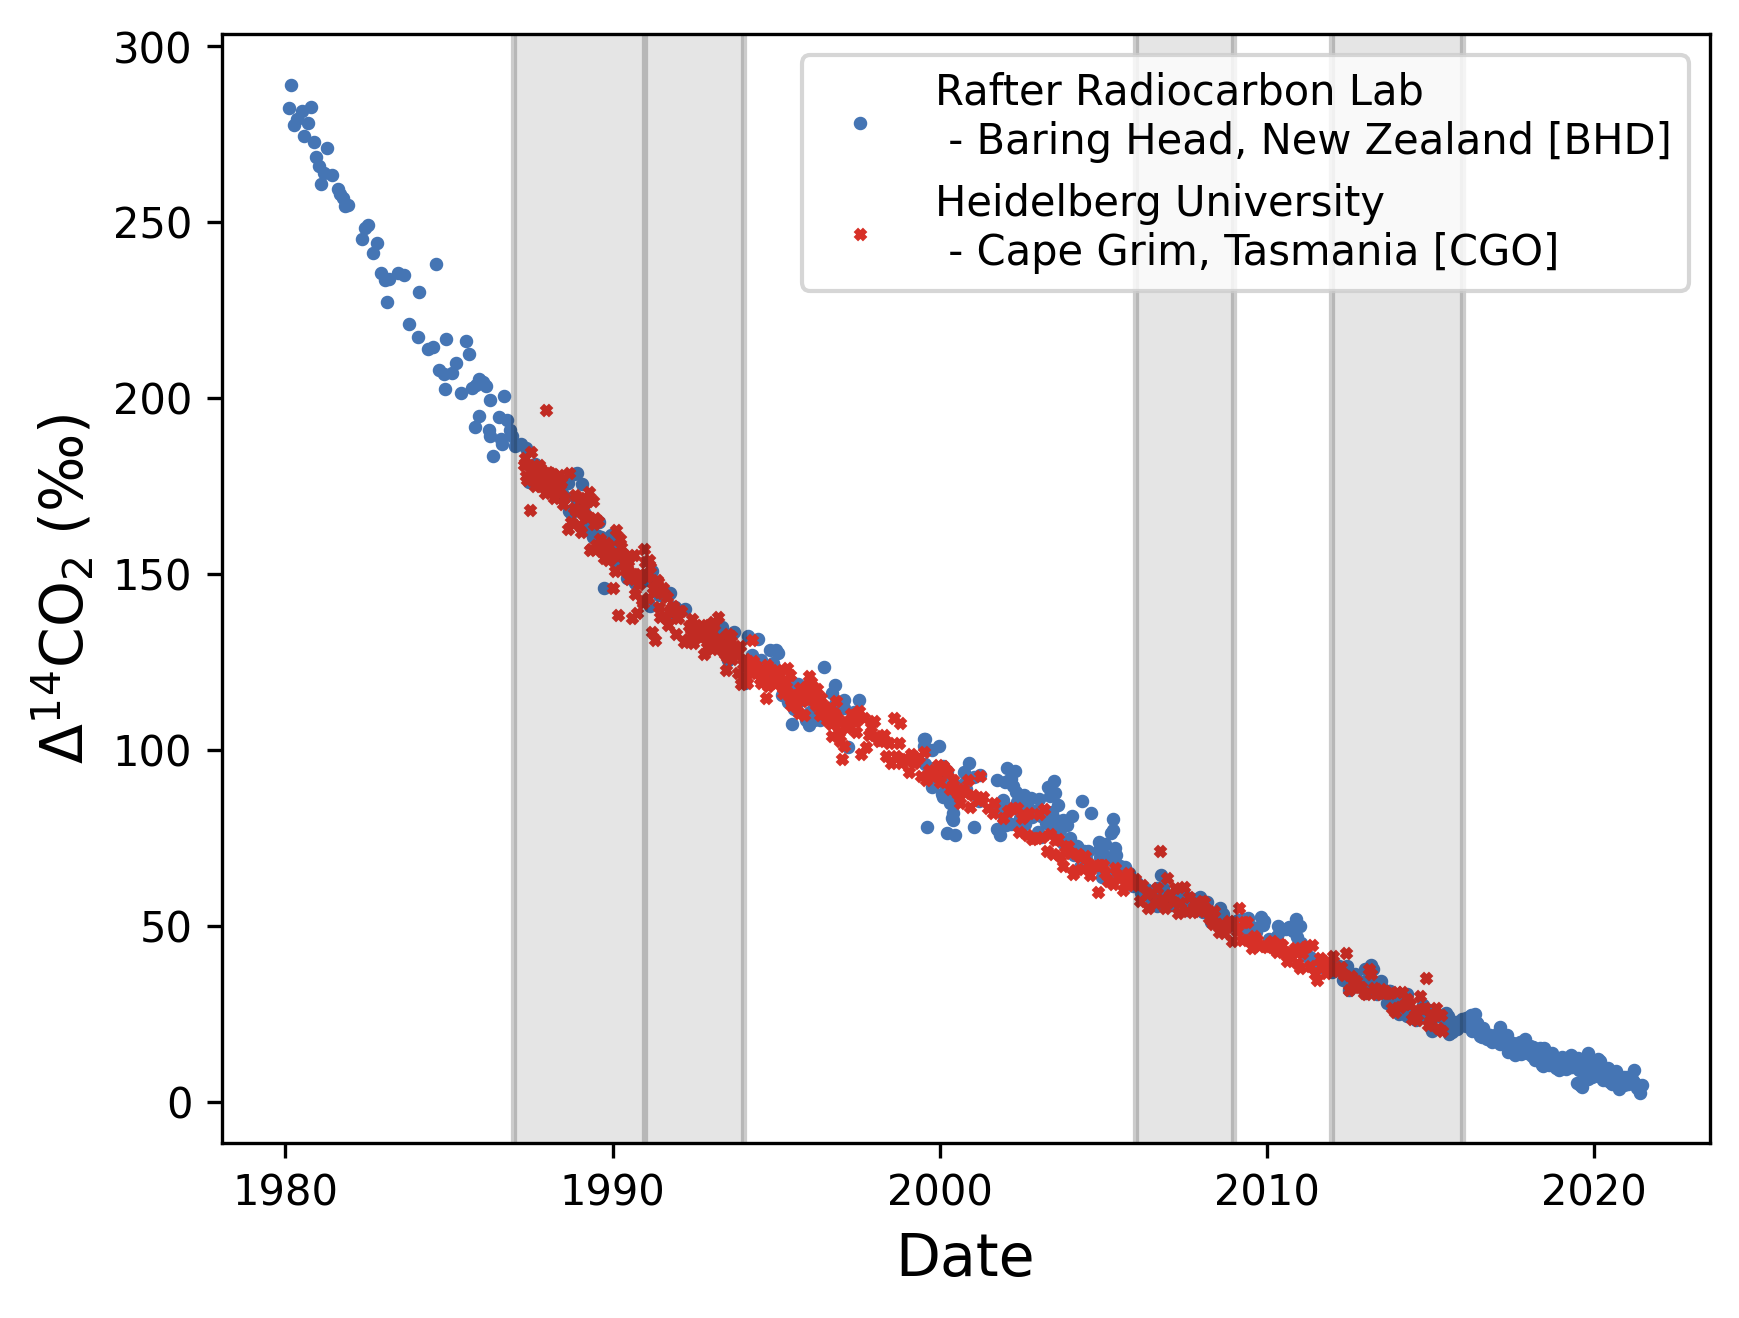
\includegraphics[width=12cm]{plots/new_test.png}
  \caption{Visual summary of available data used for intercomparison between Heidelberg University and Rafter Radiocarbon Lab. The four time intervals of focus are highlighted with background grey: 1987 - 1991, 1991 - 1994, 2006 - 2009, 2012 - 2016 }
  \label{fig:4timeintervals}
\end{figure}

\begin{figure}[htp]
    \centering
    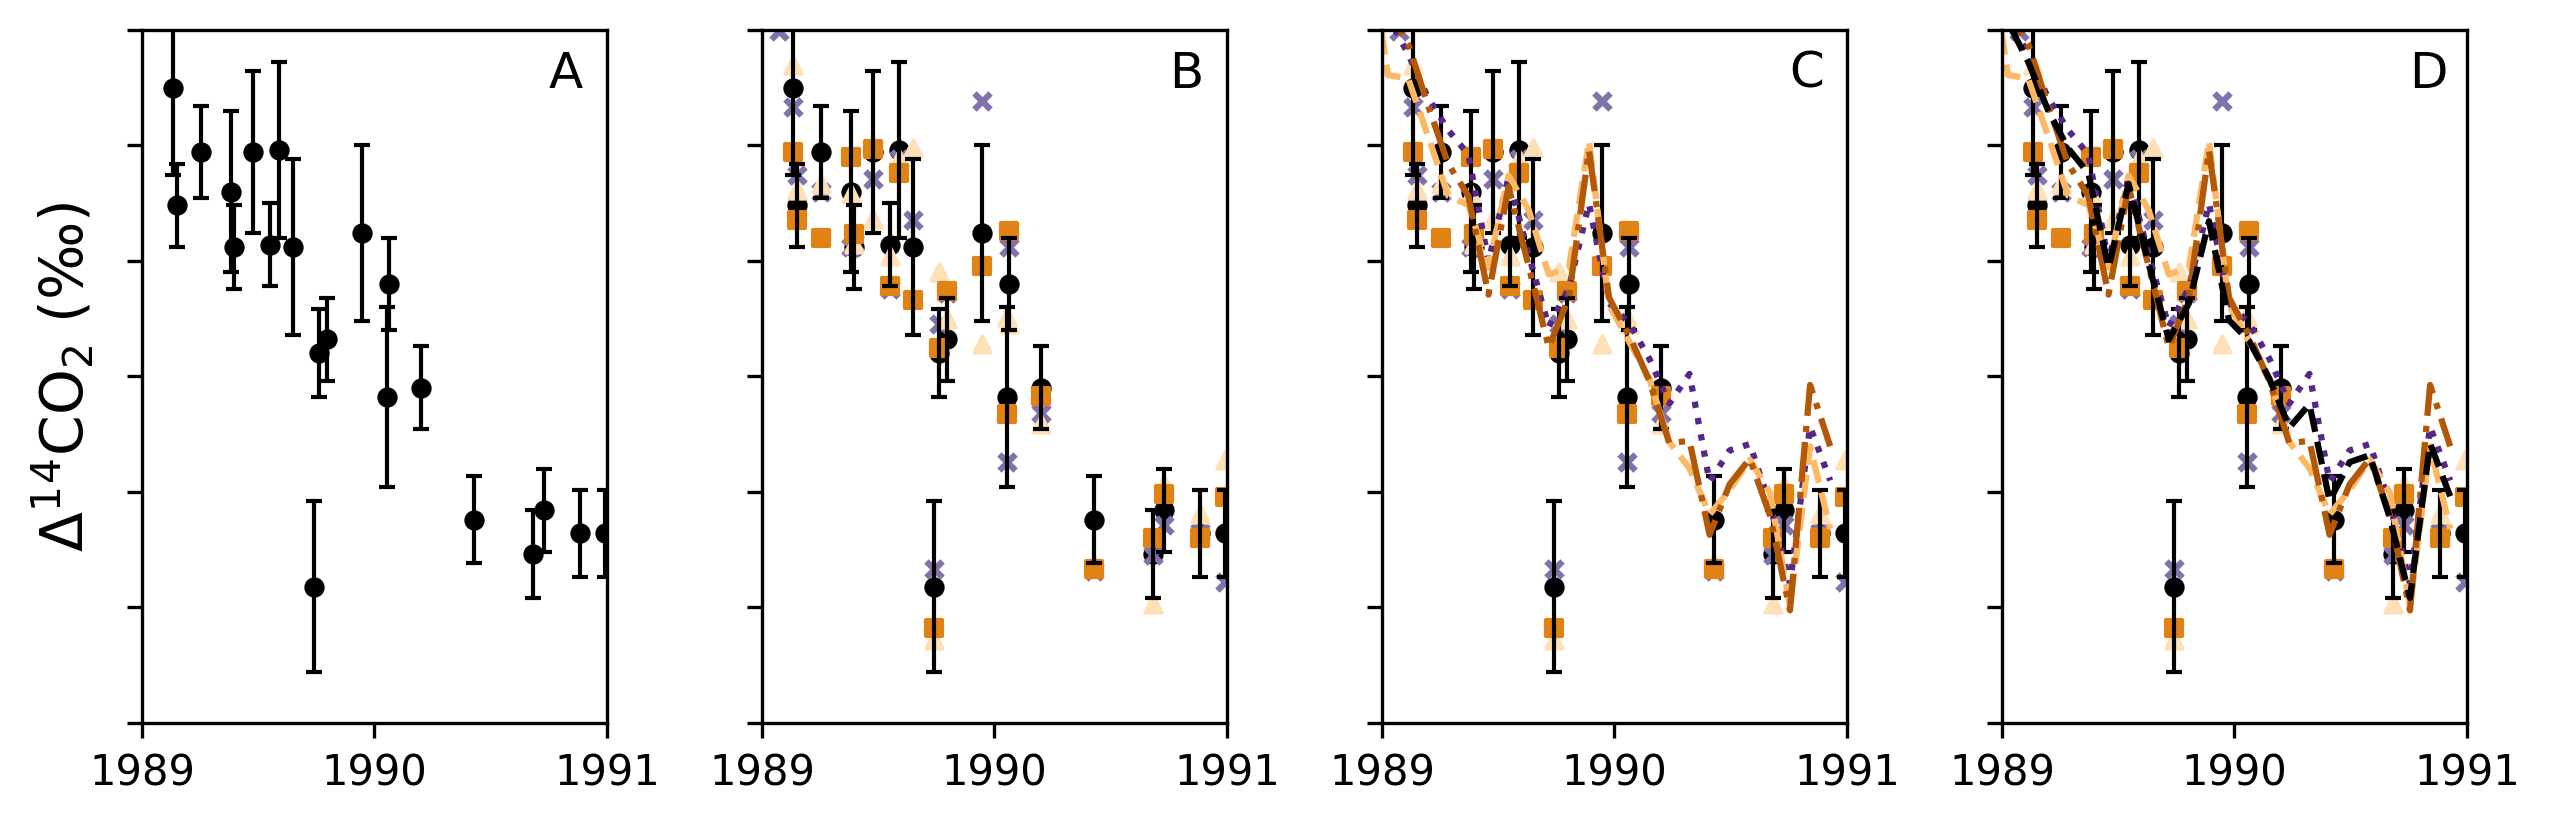
\includegraphics[width=\textwidth]{plots/DEV_FirstDraft_figureS1.png}
    \caption{Visualization of the Monte Carlo simulation to generate an uncertainty estimate about the CCGCRV curve smoothing algorithm.}
    \label{fig:montecarloexplained}
\end{figure}

\subsection{Scripps Institude of Oceaography / Lawrence Livermore National Laboratory}

RRL and Scripps Institude of Oceaography / Lawrence Livermore National Laboratory (SIO/LLNL) are compared through measurement of the same standard materials: Niwot Ridge 3 and Niwot Ridge 4 (NWT3 and NWT4). NWT3 and NWT4 are air standards from Niwot Ridge, Colorado collected in 2005 and 2006, the latter "spiked" with fossil ${CO_{2}}$. In these particular measurements, standards were graphitized and combusted at SIO and ${\Delta^{14}C}$ measured at LLNL. This intercomparison is sparse in terms of temporal overlap, with RRL measurements ranging from 2013 to 2020; and LLNL measurements encompassing March - April 2009. 
\subsection{Australian Nuclear Science and Technology Organisation (ANSTO)}

Intercomparability between ANSTO Centre for Accelerator Science and RRL ${\Delta^{14}C}$ is assesed via measurements of Kauri tree-rings. Both Institutions measured the same samples in this intercomparison.   
Where did the tree ring come from? 
How was it treated? Was it treated the same at both institutions? 





\begin{itemize}
	\item How was the sample prepared? Other details to add. 
\end{itemize}

\subsection{University of Magallanes (NEED PERMISSION)}
  
Intercomparability between University of Magallanes and RRL ${\Delta^{14}C}$ is assesed via measurements of tree-rings in Monte Tarn, Chile (53S. Samples from either institution were collected from the same site; but not the same tree. 
\begin{itemize}
	\item How was the sample prepared? Other details to add. 
\end{itemize}


\subsection{Statistical Analyses}
For intercomparisons of non-stationary time-series, such as RRL vs ANSTO, University of Magallanes, and Heidelberg University, intercomparability is assessed using paired (relative) t-tests. Comparison with SIO/LLNL uses an independent t-test. In all cases, the null hypothesis is that no difference between the institutions exists. The hypothesis is rejected if p-values are <0.01 (these are displayed in Table X). Statistical calculations were made using the Python scipy.stats library (https://docs.scipy.org/doc/scipy/reference/stats.html).





















\newpage
\section{Results/Discussion}

\subsection{RRL vs. Heidelberg University}

\begin{figure}[h!]
  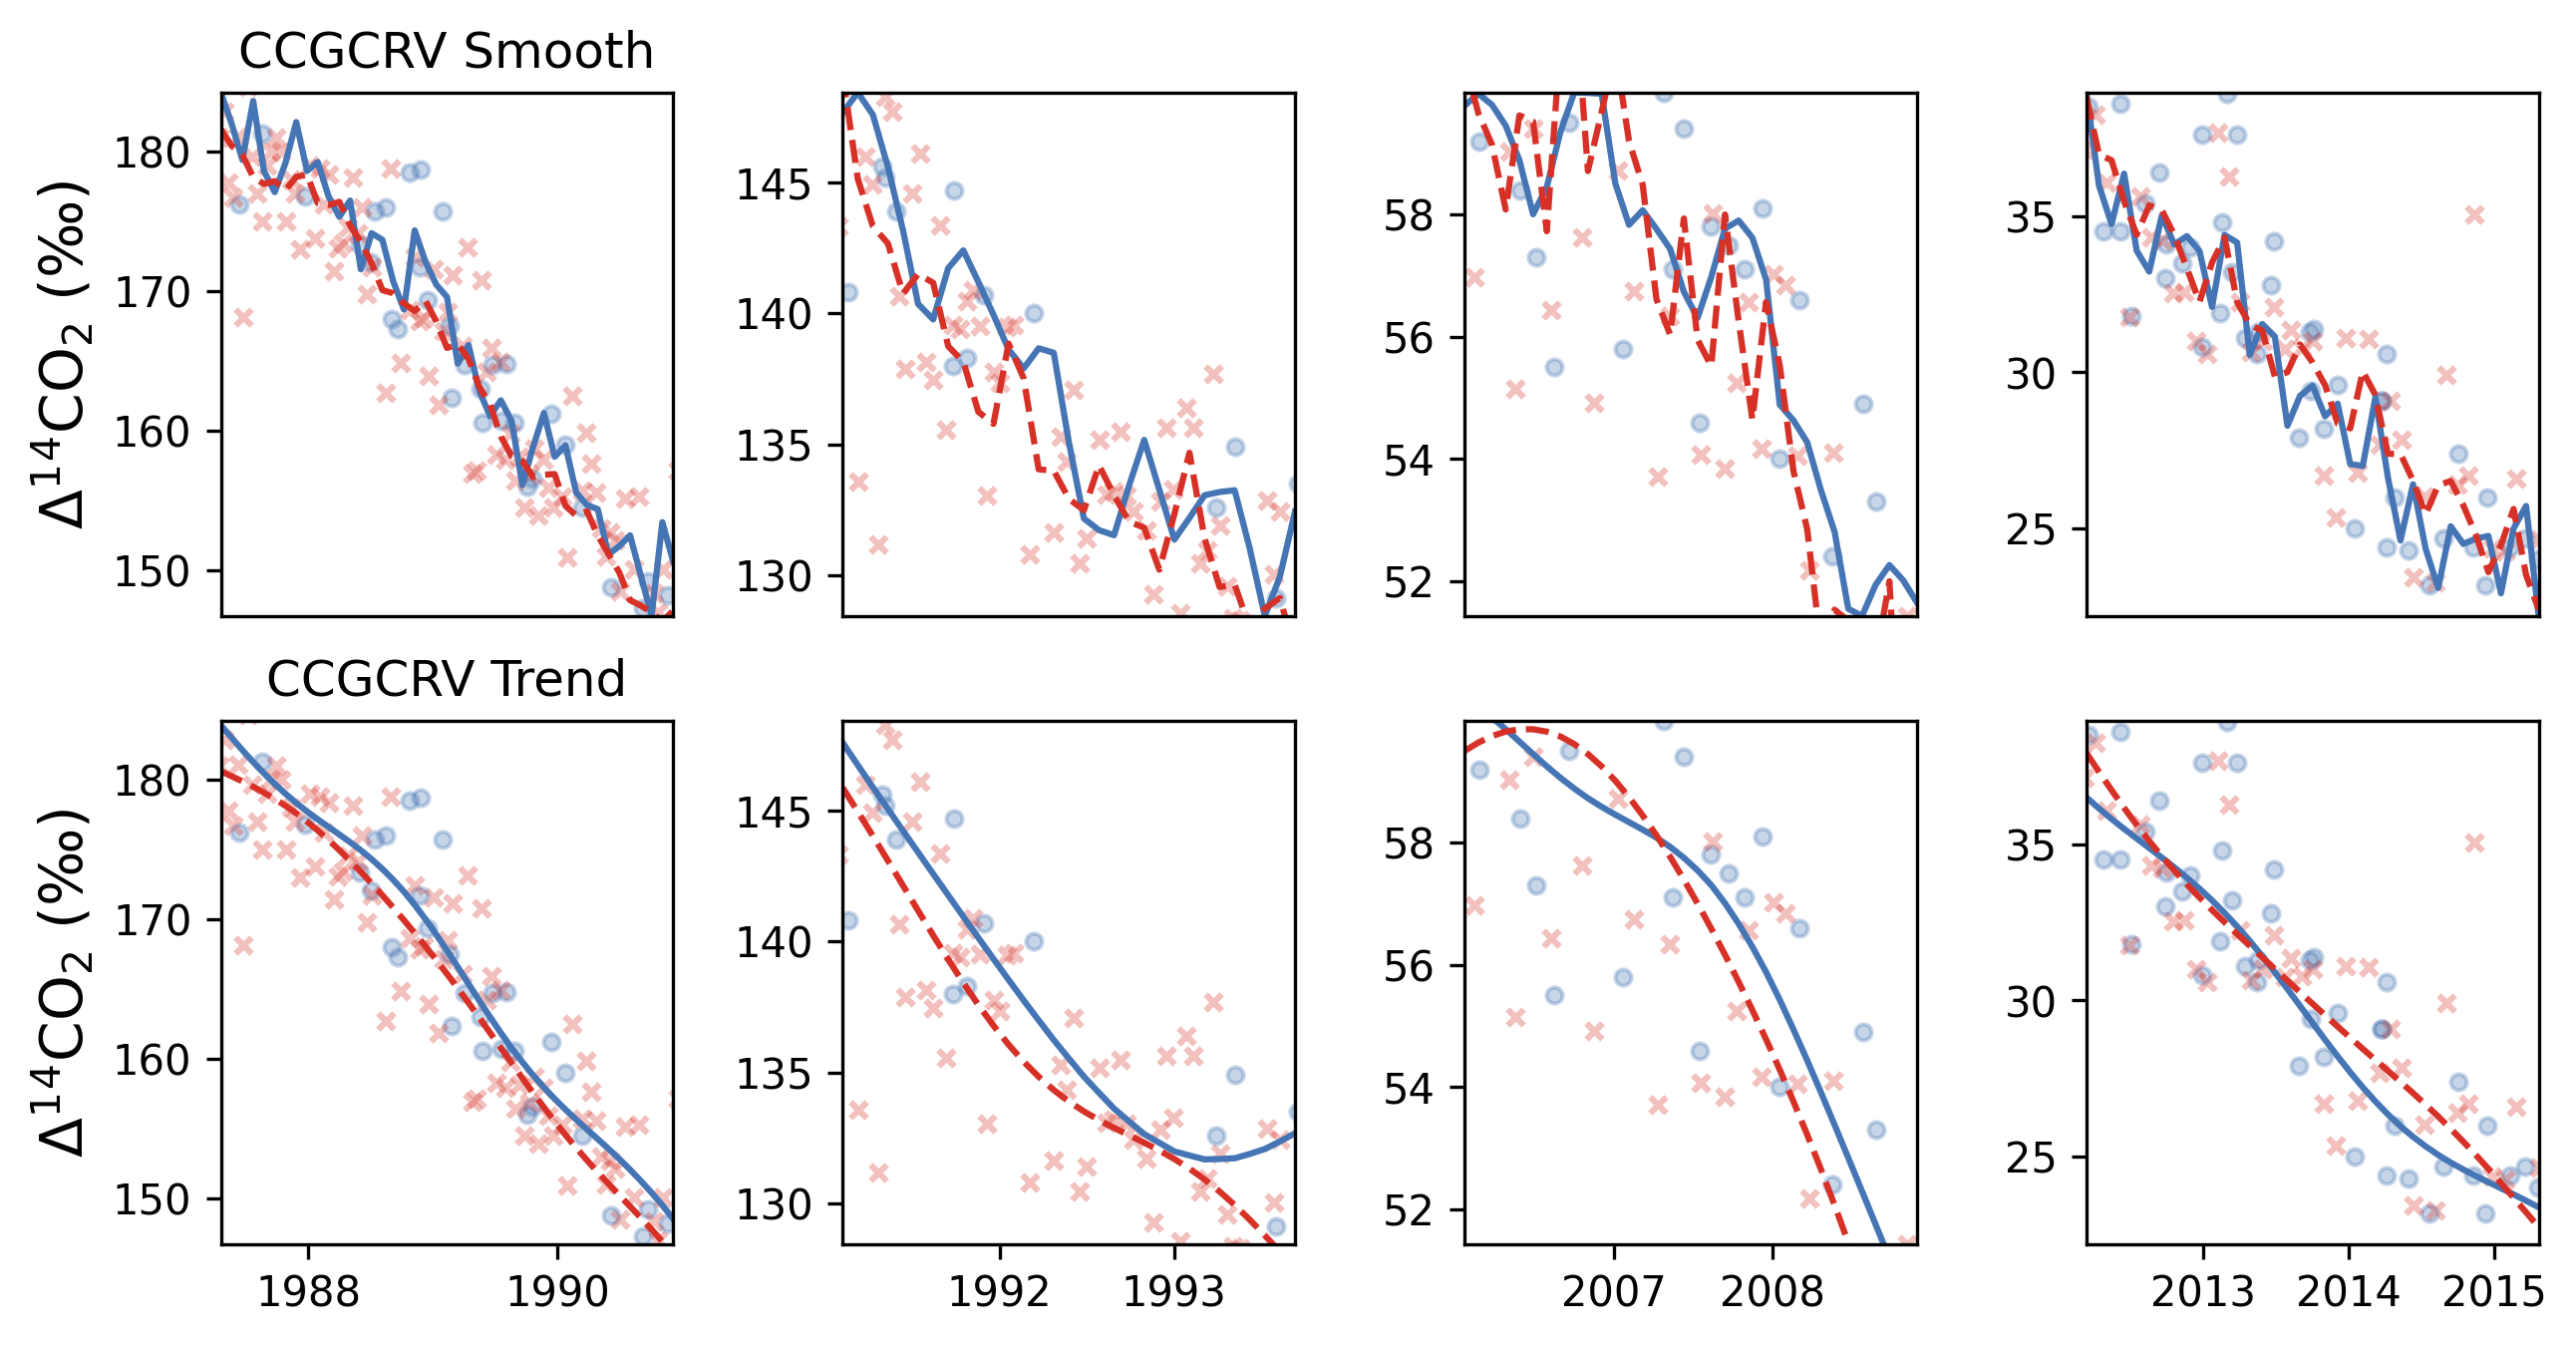
\includegraphics[width=1\textwidth]{plots/DEV_FirstDraft_figure3b_D14C.png}
  \caption{Means of Monte Carlo simulation using CCGCRV "smooth" function (top panel), and "trend" function (bottom panel) overlaid upon initial CGO and BHD data. Panel a-d represents the various time-intervals used in this intercomparison: 1987 - 1991, 1991 - 1994, 2006 - 2009, 2012 - 2016}
  \label{fig:results1}
\end{figure}
This analysis focuses on long-term trends of data, and does not focus on seasonality already explored in \cite{turnbull2017}. While \cite{turnbull2017} found CGO and BHD are consistent overall, this work takes a "deeper dive" into the trends, to understand if there are systematic offsets which might be difficult at the level we need to use D14C for carbon cycle science (2 permil) this sentence is baaaaad.

Figure shows offsets between RRL and Heidelberg University (BHD and CGO datasets, respectively) for each of the four time intervals in focus. At even steps within each interval, BHD and CGO have paired data output from the CCGCRV smoothing algorithm (mean of 10,000 Monte Carlo iterations). The difference between these data (BHD - CGO) is taken for each step, and the average difference is reported in Figure  (${\Delta\Delta^{14}C}$). Uncertainties are the 1-$\sigma$ error around the mean.
${\Delta\Delta^{14}C}$ values using the CCGCRV "smooth" and "trend" algorithm are the same within error for every case (in the rest of this section, reported data is that of CCGCRV "trend". In the period between 1987 and 1994, RRL measurements are $1.88\pm0.42$ higher than Heidelberg University (see Figure \ref{fig:results1} panel E and F), and statistically different according to paired t-tests (p-value <0.01). 
There is a step-decrease in the offset in the following intervals; D14C is  $0.55\pm0.22$\textperthousand and $-0.52\pm0.26$\textperthousand in 2006-2009 and 2012-2016, respectively. During this time period, the offset between RRL and Heidelberg University is within error of the GGMT Intercomparability goal of $0.5$\textperthousand, and the data are not statistically different. 
The following is likely responsible for the step change: 
\begin{itemize}

	\item After 2005, online 12C measurement was made possible in the EN Tandem system at GNS Science, allowing online 13C correction which dramatically decreased noise \cite{turnbull2017}
\end{itemize}

\newpage
\subsection{ANSTO and University of Magallanes}
\begin{figure}[h!]
  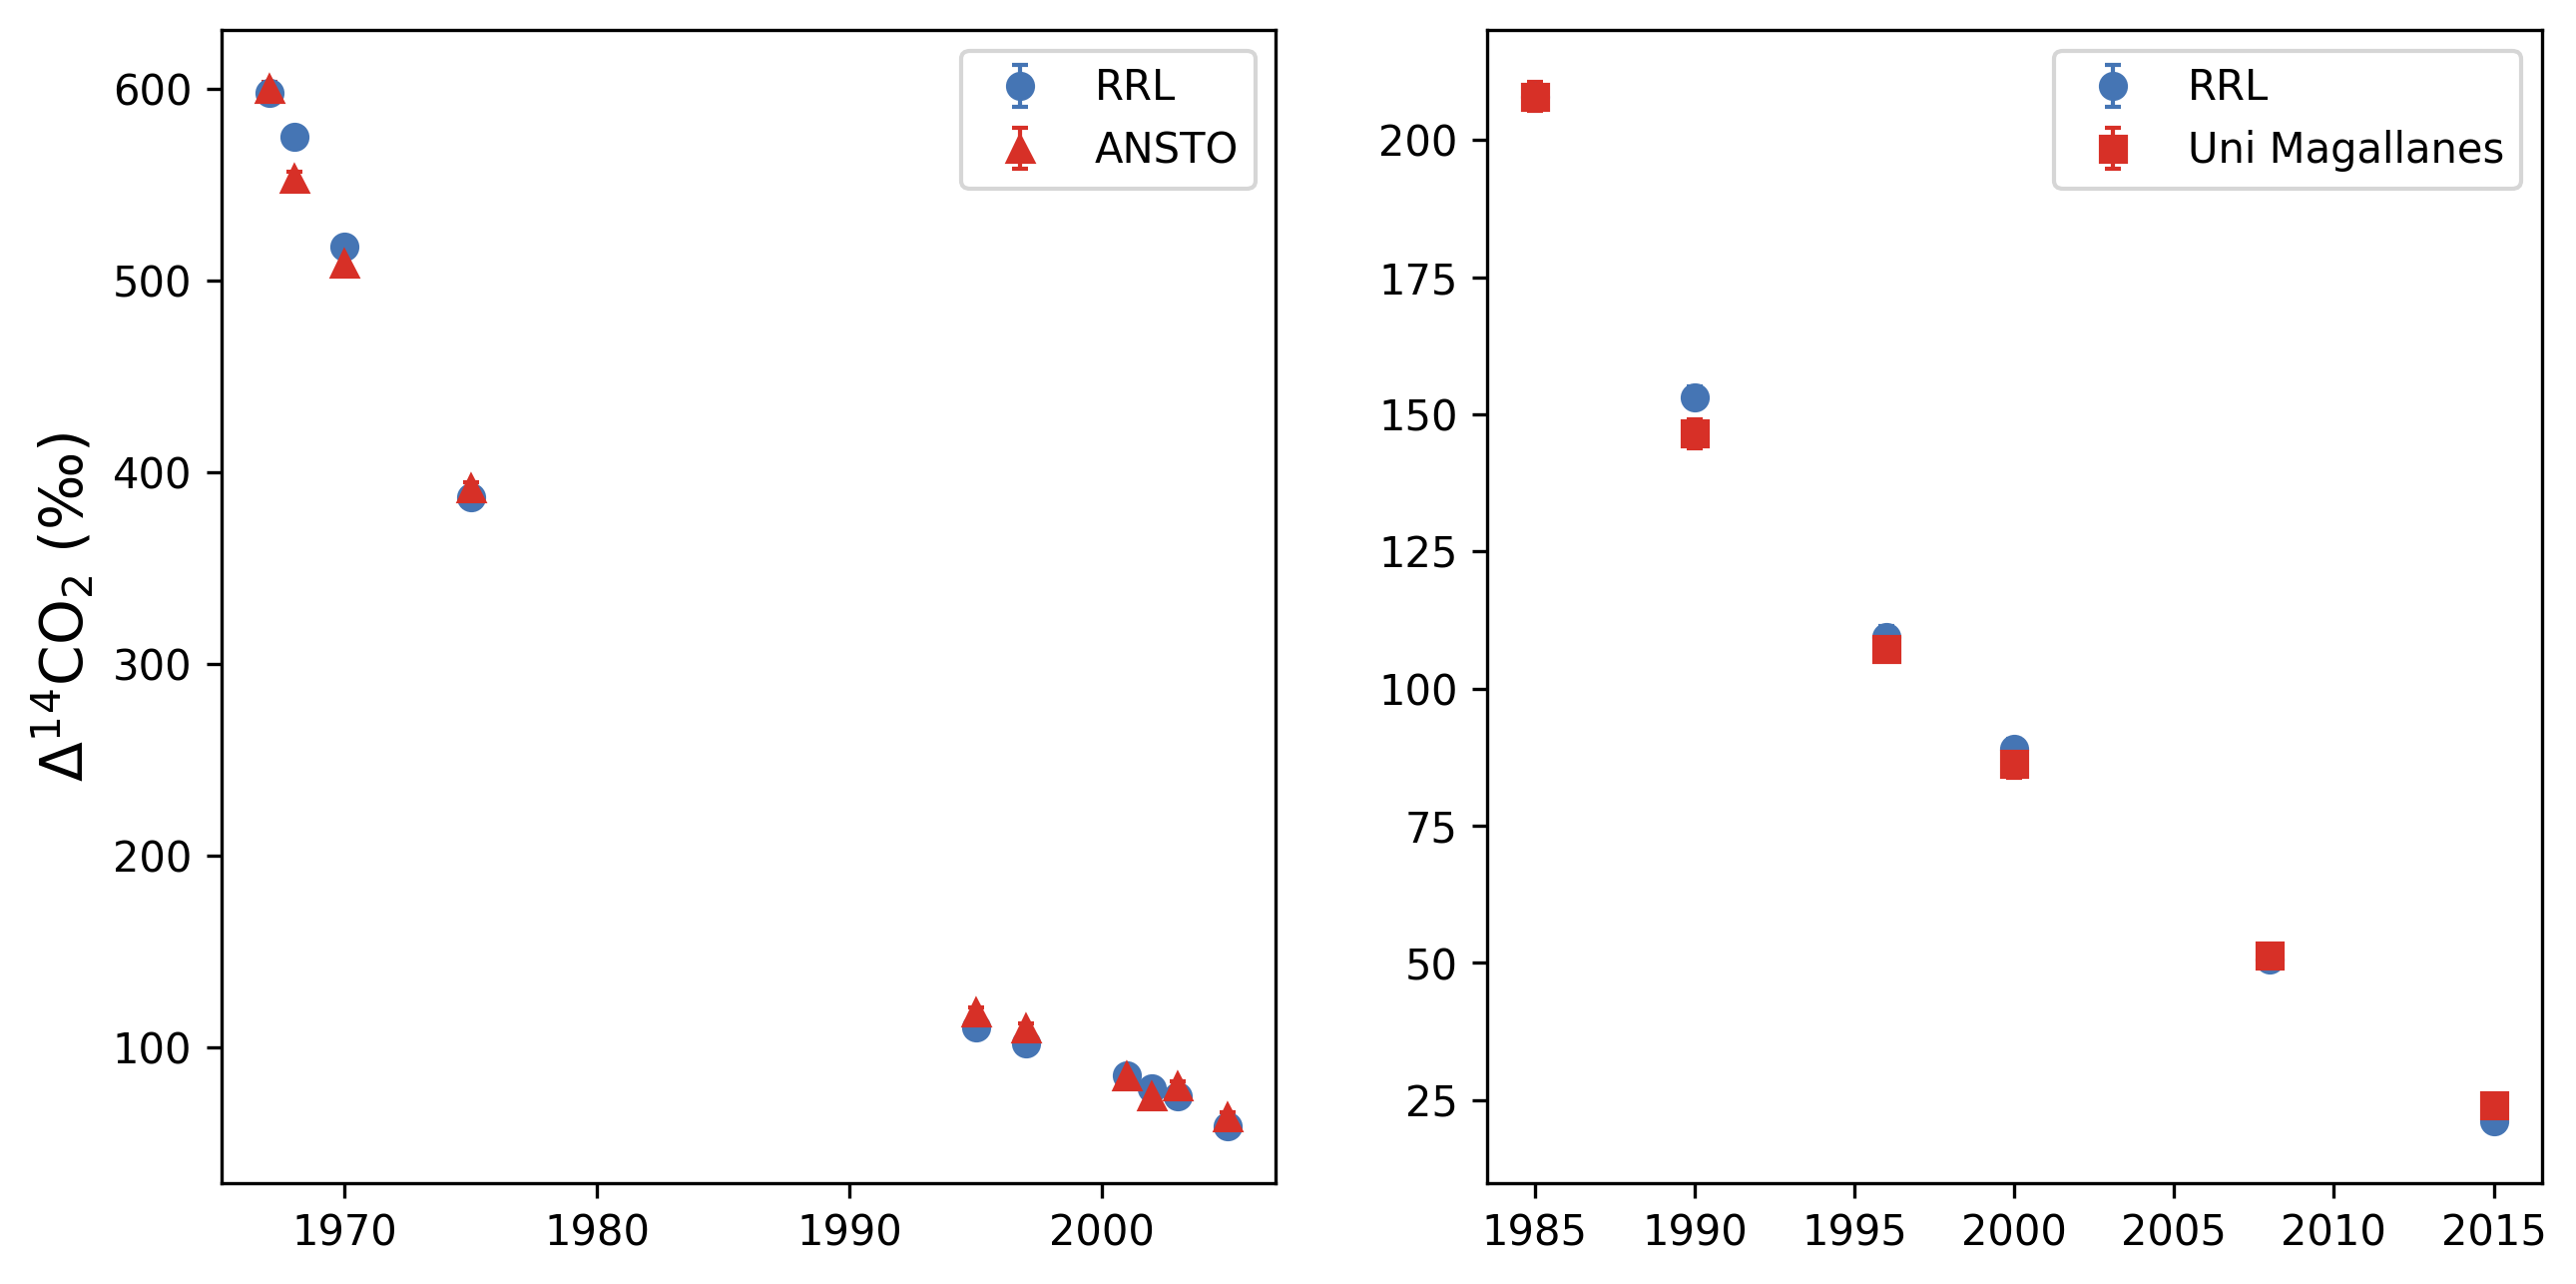
\includegraphics[width=1\textwidth]{plots/Magallanes_Ansto_comb.png}
  \caption{ADD CAPTION LATER}
  \label{fig:results1}
\end{figure}

There's no difference between the data! What a \textit{boring} section! Boo. 


\newpage
\subsection{SIO / LLNL}

\begin{figure}[h!]
  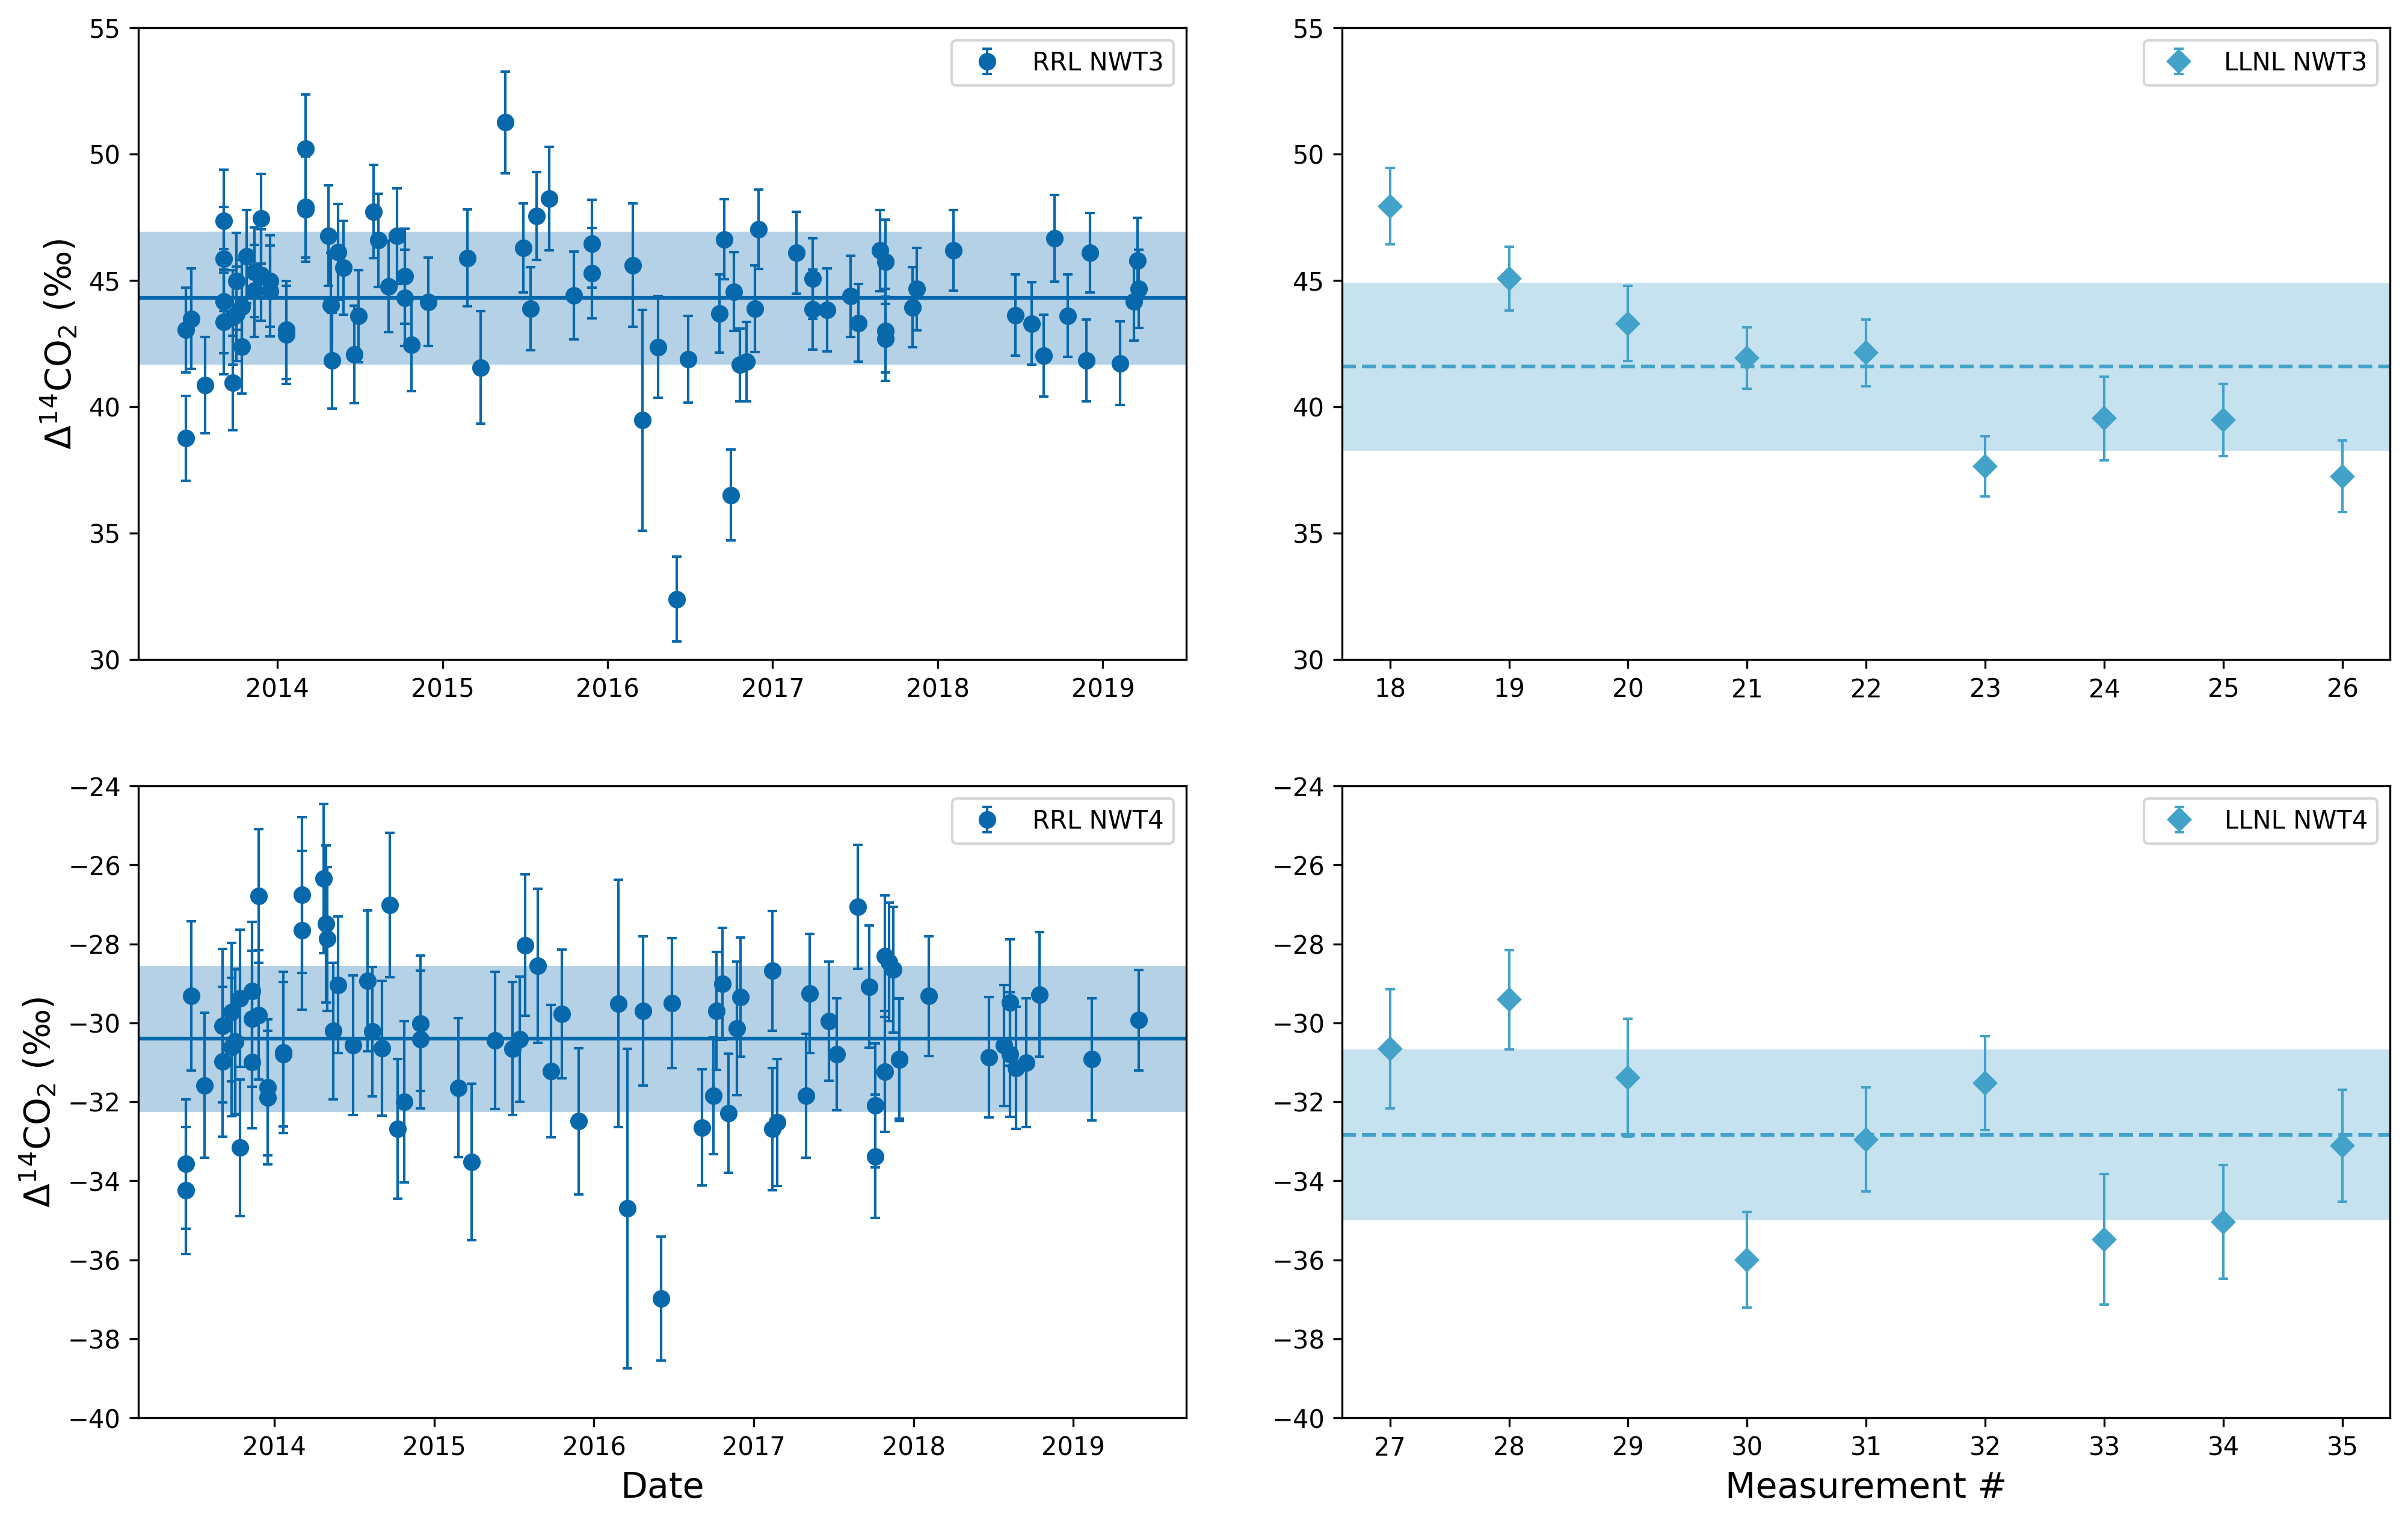
\includegraphics[width=1\textwidth]{plots/SIOLLNLvRRL.png}
  \caption{Top panel shows ${\Delta^{14}CO_{2}}$ measurements of NWT3 standard from RRL (a) and SIO/LLNL (b), respectively. Bottom panel similarly shows NWT4 standard.}
  \label{fig:siollnl}
\end{figure}

Figure \ref{fig:siollnl} shows measurements of NWT3 and NWT4 standard materials from RRL (left column) and SIO/LLNL (right column). The mean and $1-\sigma$ error of each dataset is indicated by the black bar and horizontal box. For NWT3 and NWT4 standards, RRL measurements average $2.72\pm1.14$\textperthousand and $2.44\pm0.75$\textperthousand higher than SIO/LLNL. While means are within $1-\sigma$ error of each other, independent t-tests show the data are statistically different. 
These data can be challenging to interpret as a true baseline for institutional intercomparability beacuse the avaialble datasets do not overlap in time (RRL: 2013-2020; SIO/LLNL: March-April 2009) and are of significantly different lenght (RRL: n=88; SIO/LLNL: n=9).


\newpage
\begin{tabular}{ |p{4cm}||p{2cm}|p{2cm}|p{3cm}|  }

    \hline
        Institution & ${\Delta\Delta^{14}C}$ & p-value & statistical result \\
    \hline

    (Heid. Uni) 1987-1991 & 1.75\pm0.10 &  4.9e-21 & Different          \\ 
    (Heid. Uni) 1991-1994 & 1.89\pm0.20 & 1.3e-10  & Different       \\ 
    (Heid. Uni) 2006-2009  &  0.55\pm0.14 &  6.0e-4 & Different       \\ 
    (Heid. Uni) 2012-2016  &  -0.51\pm0.10 & 2.15e-5  & Different  \\ 
    SIO/LLNL [NWT3] & 2.72\pm1.14 & 0.005 & Different \\
    SIO/LLNL [NWT4] & 2.44\pm0.75 & 4e-4 & Different \\
    ANSTO & 0.46\pm2.76 & 0.88  & Not Different \\

\hline

\end{tabular} 
\end{document}






















\newpage
\section{Conclusion}
\begin{itemize}
	\item The importance of this is: the dataset with the longest record reveals the potential variability in two institutions over time; wrt to instruments, users, and associated combustion/graphitization blanks that can all lead to small but persistent offsets that may propagate through the science. This Heidelberg intercomparison shows that in order to get meaningful understandings of the true intercomparability of institutions over time, it must be constantly repeated. 
	\item if the data with the longest available record shows not only changes, but gradients of changes in time with instrument changes, it seeds doubt in the ability to use a short term intercomparison (such as SIO/LLNL) or ANSTO, for long-term offset corrections. 
	\item Where do the offsets come from? Since normalizations to ox-1 should be the same, perhaps they come from combustion and graphitization? Perhaps they come from blank correction strategies? A good way to deal with this/ try to explore this is to have "nested" intercomparisons for example 1) we are all sent graphitze/zinc tubes and press them in house, therefore excluding combustion/graphitization blanks 2) send CO2 in breakseals (what we normally do), and 3) perhaps share blank-correction codes/excel sheets, python codes, software (Fudger, CALAMS), more widely so that users can test differences/intercomparability and edit if they see fit. 
	\item this is something we will address in upcoming iterations of intercomparison, similar to ~\cite{miller2013}. 
    \item these data are hopefully going to be used to offset correct some more data for a new work...can they be trusted? 
    
\end{itemize}
\newpage
\section{Miscellaneous}
\subsection{Acknowledgements}


\subsection{Data and materials availability}
\begin{itemize}
	\item The pre-processed data that is read into the scripts can be found in: ~\newline C:Users/clewis/IdeaProjects/GNS/InterlabComparison/output/ and can be available through GNS Science
	\item The scripts used to process said data is found at my Github page: ~\newline https://github.com/christianlewis091/scienceprojects/tree/main/InterlabComparison/scripts
\end{itemize}























\newpage
\section{Supplementary Information/Appendix}

\subsection{Site Intercomparison of Baring Head and Cape Grim}


\begin{figure}[htp]
    \centering
    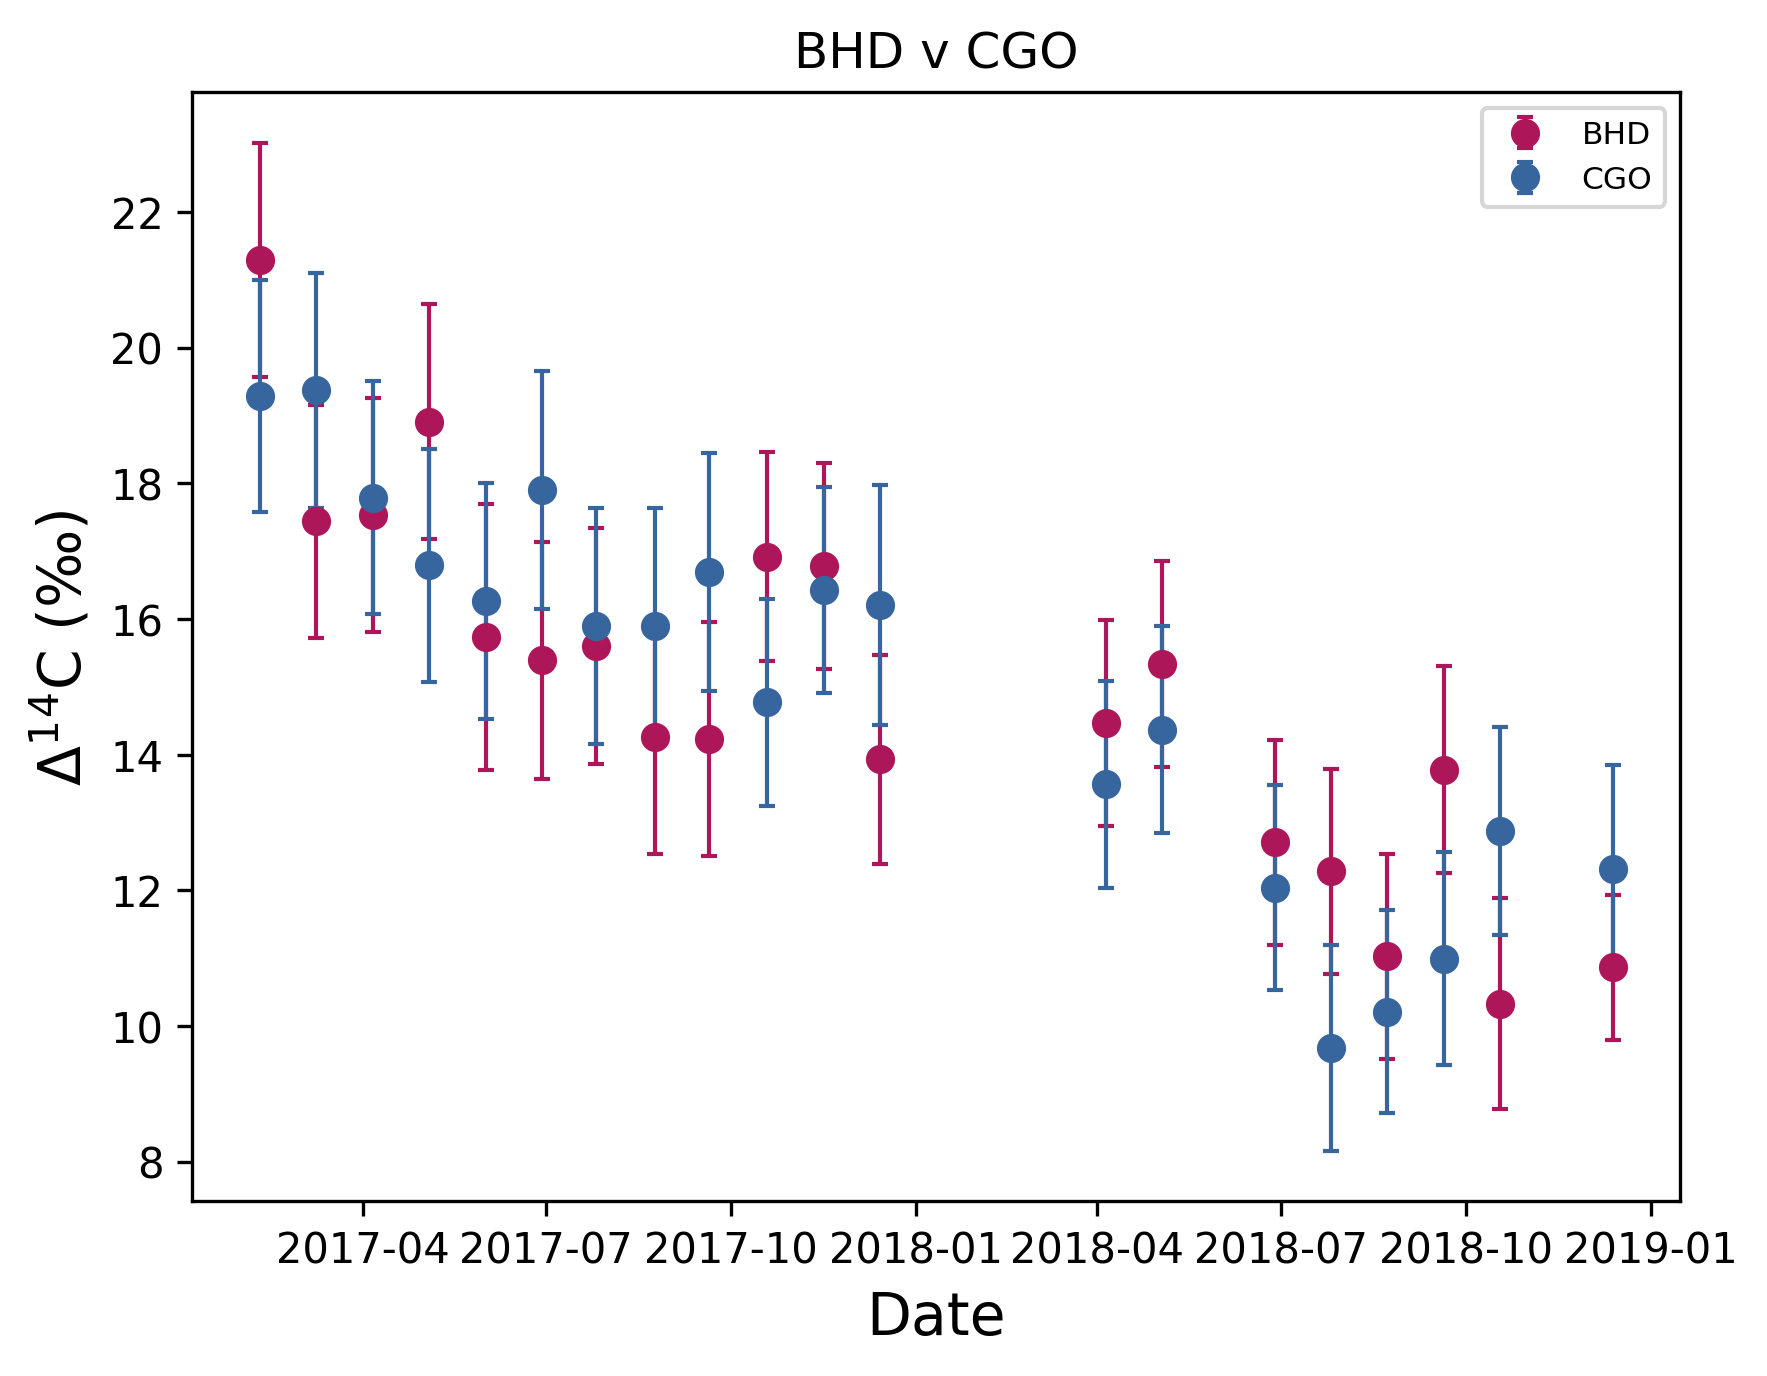
\includegraphics[width=12cm]{plots/Site_intercomparison.png}
    \caption{Intercomparison of ${\Delta^{14}CO_{2}}$ measurements  at Cape Grim, Tasmania (CGO), and Baring Head, New Zealand (BHD) collected by NIWA and measured at Rafter Radiocarbon Laboratory. Dates represent the middle of the sampling period, which differ no more than one day between sites. These data show that during the time in which data are available, no measureable difference is found between the two sites. This provides some evidence that the two sites may be considered equivalent for this intercomparability study.}
    \label{fig:bhdvcgo}
\end{figure}

\newpage
\bibliographystyle{plain}
\bibliography{bibliography.bib}



\end{document}
